\chapter{Sprint 5 -- Configuration Library and Finalization}

\setlength{\textfloatsep}{8pt plus 2pt minus 2pt}
\setlength{\floatsep}{8pt plus 2pt minus 2pt}
\setlength{\intextsep}{8pt plus 2pt minus 2pt}
\setlength{\abovecaptionskip}{4pt}
\setlength{\belowcaptionskip}{0pt}

\section*{Introduction}
\addcontentsline{toc}{section}{Introduction}

\paragraph{}After standalone generation, connected generation, and LLM enrichment were completed,
the remaining need was reuse. QA engineers often repeat the same generation scenarios during
regression testing, with only small adjustments between test runs. Recreating these configurations
manually wastes time and increases the risk of selecting inconsistent parameters.

\paragraph{}Sprint 5 therefore adds a configuration library. It allows the QA engineer to save,
overwrite, save as, import, export, inspect, search, filter, load, rename, and delete reusable
generation configurations. The sprint also finalizes connected-mode safeguards so that saved
connected scenarios are loaded only when they are compatible with the grabbed data context.

\section{Sprint Backlog}

\paragraph{}The backlog of Sprint 5 focuses on scenario reuse, connected compatibility checks, and
final workflow safeguards. Table~\ref{tab:sprint5-backlog} summarizes the planned work.

\small
\renewcommand{\arraystretch}{1.05}
\begin{longtable}{|Q{0.07\linewidth}|P{0.29\linewidth}|P{0.42\linewidth}|Q{0.12\linewidth}|}
\caption{Sprint 5 backlog}
\label{tab:sprint5-backlog} \\
\hline
\textbf{ID} & \textbf{Task} & \textbf{Description} & \textbf{Estimate} \\
\hline
\endfirsthead
\multicolumn{4}{r}{\tablename\ \thetable{} -- \textit{continued from previous page}} \\
\hline
\textbf{ID} & \textbf{Task} & \textbf{Description} & \textbf{Estimate} \\
\hline
\endhead
\hline
\multicolumn{4}{r}{\textit{continued on next page}} \\
\endfoot
\hline
\endlastfoot
T5-1 & Define saved configuration entity & Store the name, description, mode, schema version, connected grab mode, JSON payload, creation date, and update date. & 1 day \\
\hline
T5-2 & Implement library API & Provide create, list, find, update, delete, compatible connected lookup, JSON validation, and overwrite support. & 2 days \\
\hline
T5-3 & Add standalone save and load & Save a standalone configuration and restore it into the standalone workflow. & 1 day \\
\hline
T5-4 & Add connected save and load & Save connected scenarios with their grab mode and load only compatible configurations. & 2 days \\
\hline
T5-5 & Build library page & Add browsing, search, mode filtering, pagination, details, import/export, renaming, deletion, empty state, and error state. & 3 days \\
\hline
T5-6 & Add save lifecycle controls & Track the loaded configuration source, overwrite it directly, or create a separate copy with Save As. & 2 days \\
\hline
T5-7 & Finalize navigation safeguards & Preserve local state and confirm disconnection when leaving an active connected session. & 1 day \\
\hline
T5-8 & Validate the full workflow & Check standalone, connected, enrichment, library, JSON exchange, and SQL export flows end to end. & 1 day \\
\hline
\end{longtable}
\normalsize
\renewcommand{\arraystretch}{1}

\section{Sprint Specification}

\paragraph{}The configuration library is shared by standalone and connected modes. Standalone
configurations can be restored directly. Connected configurations require additional checks because
they depend on the grabbed accounts, account groups, or securities selected in the active connected
session.

\subsection{Use Case Refinement}

\paragraph{}Figure~\ref{fig:usecase-library} presents the refined use case diagram of the
configuration library, while Table~\ref{tab:sprint5-refined-usecases} summarizes each action.

\begin{figure}[!htbp]
\centering
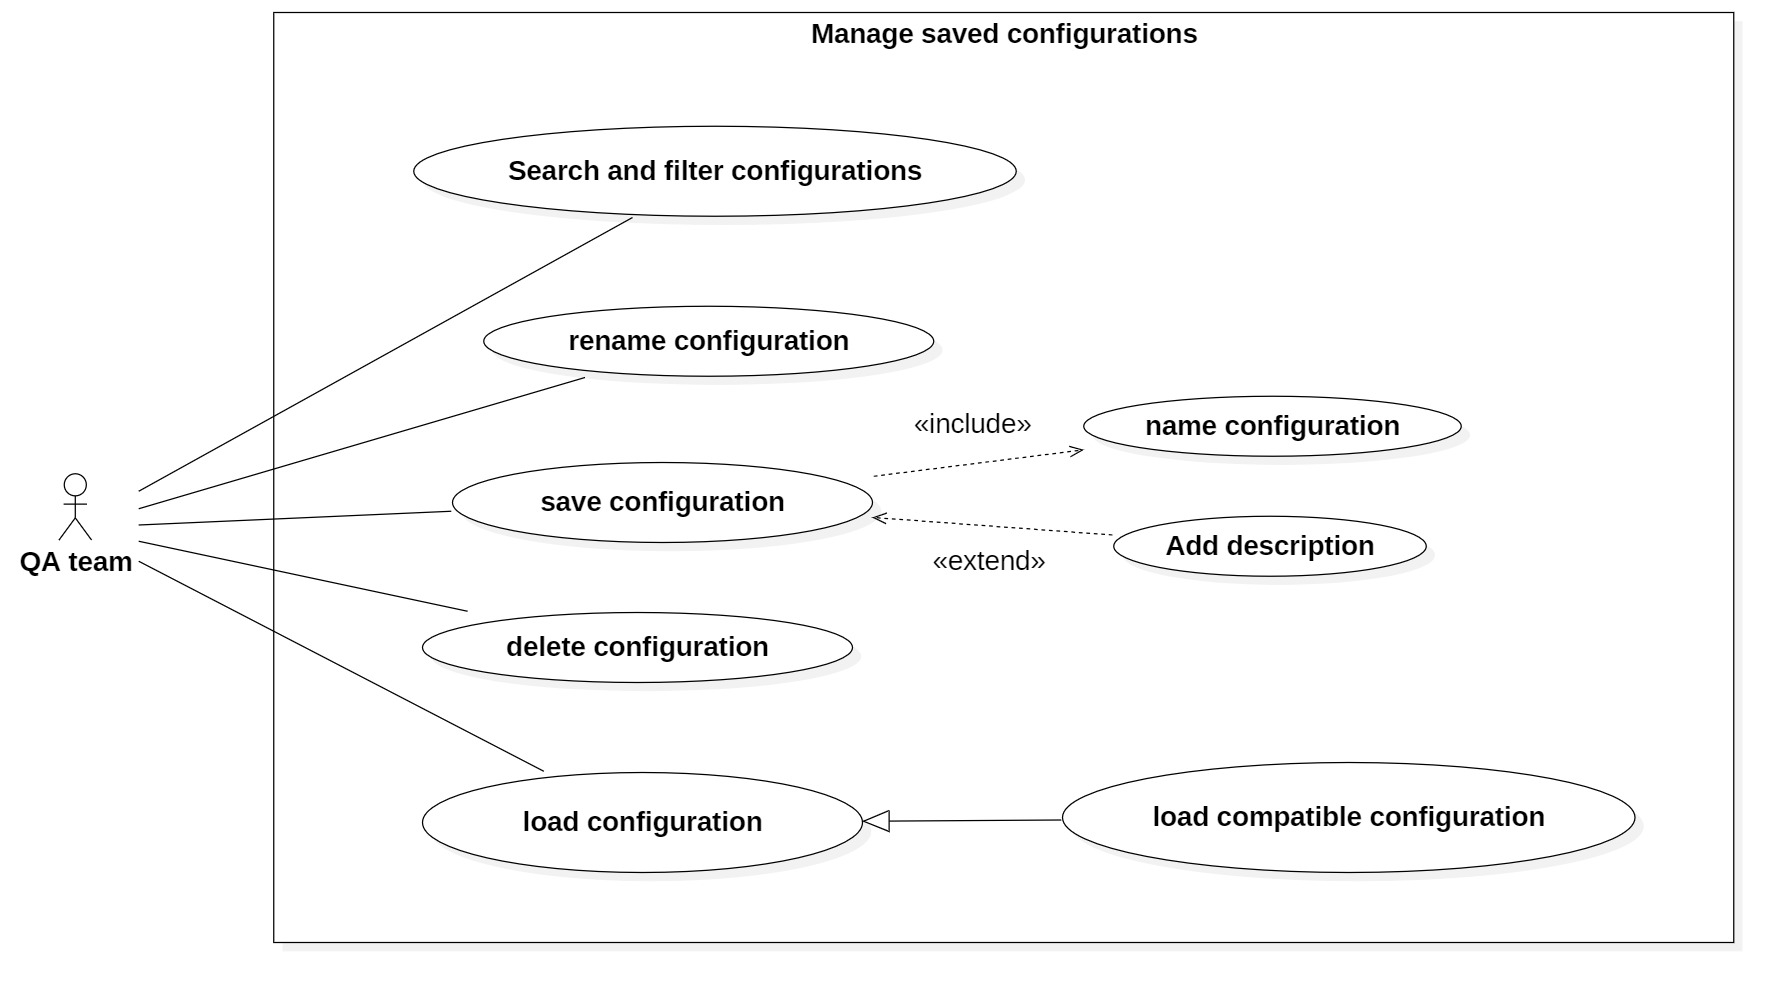
\includegraphics[width=0.95\textwidth]{img/usecase-config-library.jpg}
\caption{Refined use case diagram of the configuration library}
\label{fig:usecase-library}
\end{figure}

\renewcommand{\arraystretch}{1.15}
\begin{longtable}{|P{0.27\linewidth}|P{0.23\linewidth}|P{0.40\linewidth}|}
\caption{Refined use cases of Sprint 5}
\label{tab:sprint5-refined-usecases} \\
\hline
\textbf{Refined use case} & \textbf{Actor} & \textbf{Goal} \\
\hline
\endfirsthead
\multicolumn{3}{r}{\tablename\ \thetable{} -- \textit{continued from previous page}} \\
\hline
\textbf{Refined use case} & \textbf{Actor} & \textbf{Goal} \\
\hline
\endhead
\hline
\multicolumn{3}{r}{\textit{continued on next page}} \\
\endfoot
\hline
\endlastfoot
Save configuration & QA Engineer & Store the current standalone or connected scenario for later reuse. \\
\hline
Overwrite loaded configuration & QA Engineer & Replace the payload of the currently loaded saved scenario. \\
\hline
Save as configuration & QA Engineer & Create a new saved scenario from a loaded configuration. \\
\hline
Browse configurations & QA Engineer & View saved scenarios with their mode, description, and dates. \\
\hline
Search and filter & QA Engineer & Find saved scenarios by name or mode. \\
\hline
View configuration details & QA Engineer & Inspect the main content of a saved scenario before loading it. \\
\hline
Load standalone configuration & QA Engineer & Restore a saved standalone scenario into the standalone workflow. \\
\hline
Load connected configuration & QA Engineer & Restore a saved connected scenario only when it matches the current grabbed context. \\
\hline
Import configuration & QA Engineer & Add a saved configuration from a JSON export file. \\
\hline
Export configuration & QA Engineer & Download a saved configuration as a reusable JSON file. \\
\hline
Rename configuration & QA Engineer & Update the name of a saved scenario. \\
\hline
Delete configuration & QA Engineer & Remove an obsolete scenario after confirmation. \\
\hline
Leave connected session safely & QA Engineer & Avoid losing or mixing active connected context when navigating away. \\
\hline
\end{longtable}
\renewcommand{\arraystretch}{1}

\subsection{Textual Use Case Description}

\renewcommand{\arraystretch}{1.15}
\begin{longtable}{|P{0.24\linewidth}|P{0.66\linewidth}|}
\caption{Textual description of the configuration library use case}
\label{tab:library-usecase-description} \\
\hline
\textbf{Element} & \textbf{Description} \\
\hline
\endfirsthead
\multicolumn{2}{r}{\tablename\ \thetable{} -- \textit{continued from previous page}} \\
\hline
\textbf{Element} & \textbf{Description} \\
\hline
\endhead
\hline
\multicolumn{2}{r}{\textit{continued on next page}} \\
\endfoot
\hline
\endlastfoot
Use case & Manage reusable standalone and connected generation configurations. \\
\hline
Actor & QA Engineer. \\
\hline
Preconditions & The application is available and the QA engineer has a configuration to save or an existing entry to load. \\
\hline
Postconditions & The configuration is saved, loaded, renamed, deleted, filtered, or rejected when incompatible. \\
\hline
Main scenario &
\begin{enumerate}[leftmargin=*,nosep]
    \item The QA engineer saves a generation configuration with a name and optional description.
    \item The backend validates the name, mode, schema version, connected grab mode, and JSON payload.
    \item The configuration is stored in the local configuration library.
    \item The QA engineer opens the library page and searches or filters saved scenarios.
    \item The QA engineer expands a saved card to inspect reference date, enabled sections, schema version, and estimated rows.
    \item The QA engineer loads, renames, exports, overwrites, or deletes a saved configuration.
    \item If a loaded configuration is modified, the QA engineer can overwrite it directly or save it as a new scenario.
    \item The system applies the action and updates the visible library state.
\end{enumerate} \\
\hline
Import and export rules &
\begin{itemize}[leftmargin=*,nosep]
    \item Exported files use a typed JSON wrapper with export date, schema version, metadata, and configuration data.
    \item Imported files must be valid JSON and must match a supported configuration export format.
    \item Imported connected configurations must include a valid connected grab mode.
    \item Schema version is stored with the saved entry to support future payload evolution.
\end{itemize} \\
\hline
Compatibility rules &
\begin{itemize}[leftmargin=*,nosep]
    \item Standalone configurations can be loaded directly into standalone mode.
    \item Connected configurations are linked to a grab mode: accounts, securities, or accounts and securities.
    \item Connected configurations are sanitized before saving so generated accounts or securities are not duplicated when they already come from grabbed data.
    \item Connected loading is disabled when the saved scenario conflicts with the current grabbed data context.
\end{itemize} \\
\hline
Exception scenario &
\begin{itemize}[leftmargin=*,nosep]
    \item If the name is empty or already used, saving or renaming is rejected and an error message is shown.
    \item If the schema version is invalid, the backend rejects the save or overwrite request.
    \item If the JSON payload is missing, malformed, or does not match the expected standalone or connected structure, the backend rejects the saved configuration.
    \item If an imported file is not a supported configuration export, the interface rejects the import.
    \item If a connected configuration is incompatible, the load action is disabled and the reason is displayed.
    \item If the library API is unreachable, the interface displays an error state and offers retry.
    \item If the QA engineer leaves an active connected session, a confirmation dialog is displayed before disconnecting.
\end{itemize} \\
\hline
\end{longtable}
\renewcommand{\arraystretch}{1}

\paragraph{}In standalone mode, saving and loading is direct because the whole scenario is generated
from the saved parameters. In connected mode, the saved configuration depends on the data grabbed
from SQL Server. For this reason, connected configurations store their grab mode and are loaded only
when the current connected session provides a compatible context.

\renewcommand{\arraystretch}{1.15}
\begin{longtable}{|P{0.24\linewidth}|P{0.66\linewidth}|}
\caption{Textual description of the connected configuration save and load use case}
\label{tab:connected-library-usecase-description} \\
\hline
\textbf{Element} & \textbf{Description} \\
\hline
\endfirsthead
\multicolumn{2}{r}{\tablename\ \thetable{} -- \textit{continued from previous page}} \\
\hline
\textbf{Element} & \textbf{Description} \\
\hline
\endhead
\hline
\multicolumn{2}{r}{\textit{continued on next page}} \\
\endfoot
\hline
\endlastfoot
Use case & Save and load a connected generation configuration. \\
\hline
Actor & QA Engineer. \\
\hline
Preconditions & A connected session is active and the QA engineer has grabbed accounts, securities, or both from SQL Server. \\
\hline
Main scenario &
\begin{enumerate}[leftmargin=*,nosep]
    \item The QA engineer prepares a connected generation configuration using the grabbed data.
    \item The application saves the configuration with its mode, schema version, JSON payload, and connected grab mode.
    \item Before saving, generated sections that would duplicate grabbed accounts or securities are sanitized.
    \item Later, the QA engineer opens the library from connected mode.
    \item The application compares the saved grab mode with the current grabbed context.
    \item Compatible configurations can be loaded into the connected workflow.
    \item Incompatible configurations stay disabled and the interface displays the reason.
\end{enumerate} \\
\hline
Difference from standalone & Standalone configurations are self-contained and can be loaded directly. Connected configurations are context-dependent because their generated output must remain coherent with the records already grabbed from SQL Server. \\
\hline
Postconditions & The connected configuration is restored only when it matches the active connected context; otherwise, it is rejected before loading. \\
\hline
Exception scenarios &
\begin{itemize}[leftmargin=*,nosep]
    \item The saved grab mode does not match the active connected session.
    \item The saved payload is malformed or uses an unsupported schema version.
    \item The current connected session does not contain the data required by the saved scenario.
\end{itemize} \\
\hline
\end{longtable}
\renewcommand{\arraystretch}{1}

\section{Sprint Design}

\paragraph{}The design separates storage from workflow usage. The backend owns persistence, schema
versioning, and payload validation. The frontend owns the library cards, saved-scenario restoration,
Save/Save As behavior, import/export, compatibility feedback, and navigation safeguards.

\paragraph{}SQLite was selected for the configuration library because the saved scenarios are local
application data, not business data from Longview. It gives the application persistent storage without
requiring an additional database server, keeps installation simple for the QA engineer, and is
sufficient for the small volume of saved JSON configurations managed by this feature.

\subsection{Activity Diagram}

\paragraph{}Figure~\ref{fig:activity-library} presents the activity diagram of the configuration
library. It summarizes the main decisions of this sprint: saving or overwriting a scenario, loading
standalone configurations directly, checking connected compatibility before loading connected
configurations, and supporting JSON import and export.

\begin{figure}[!htbp]
\centering
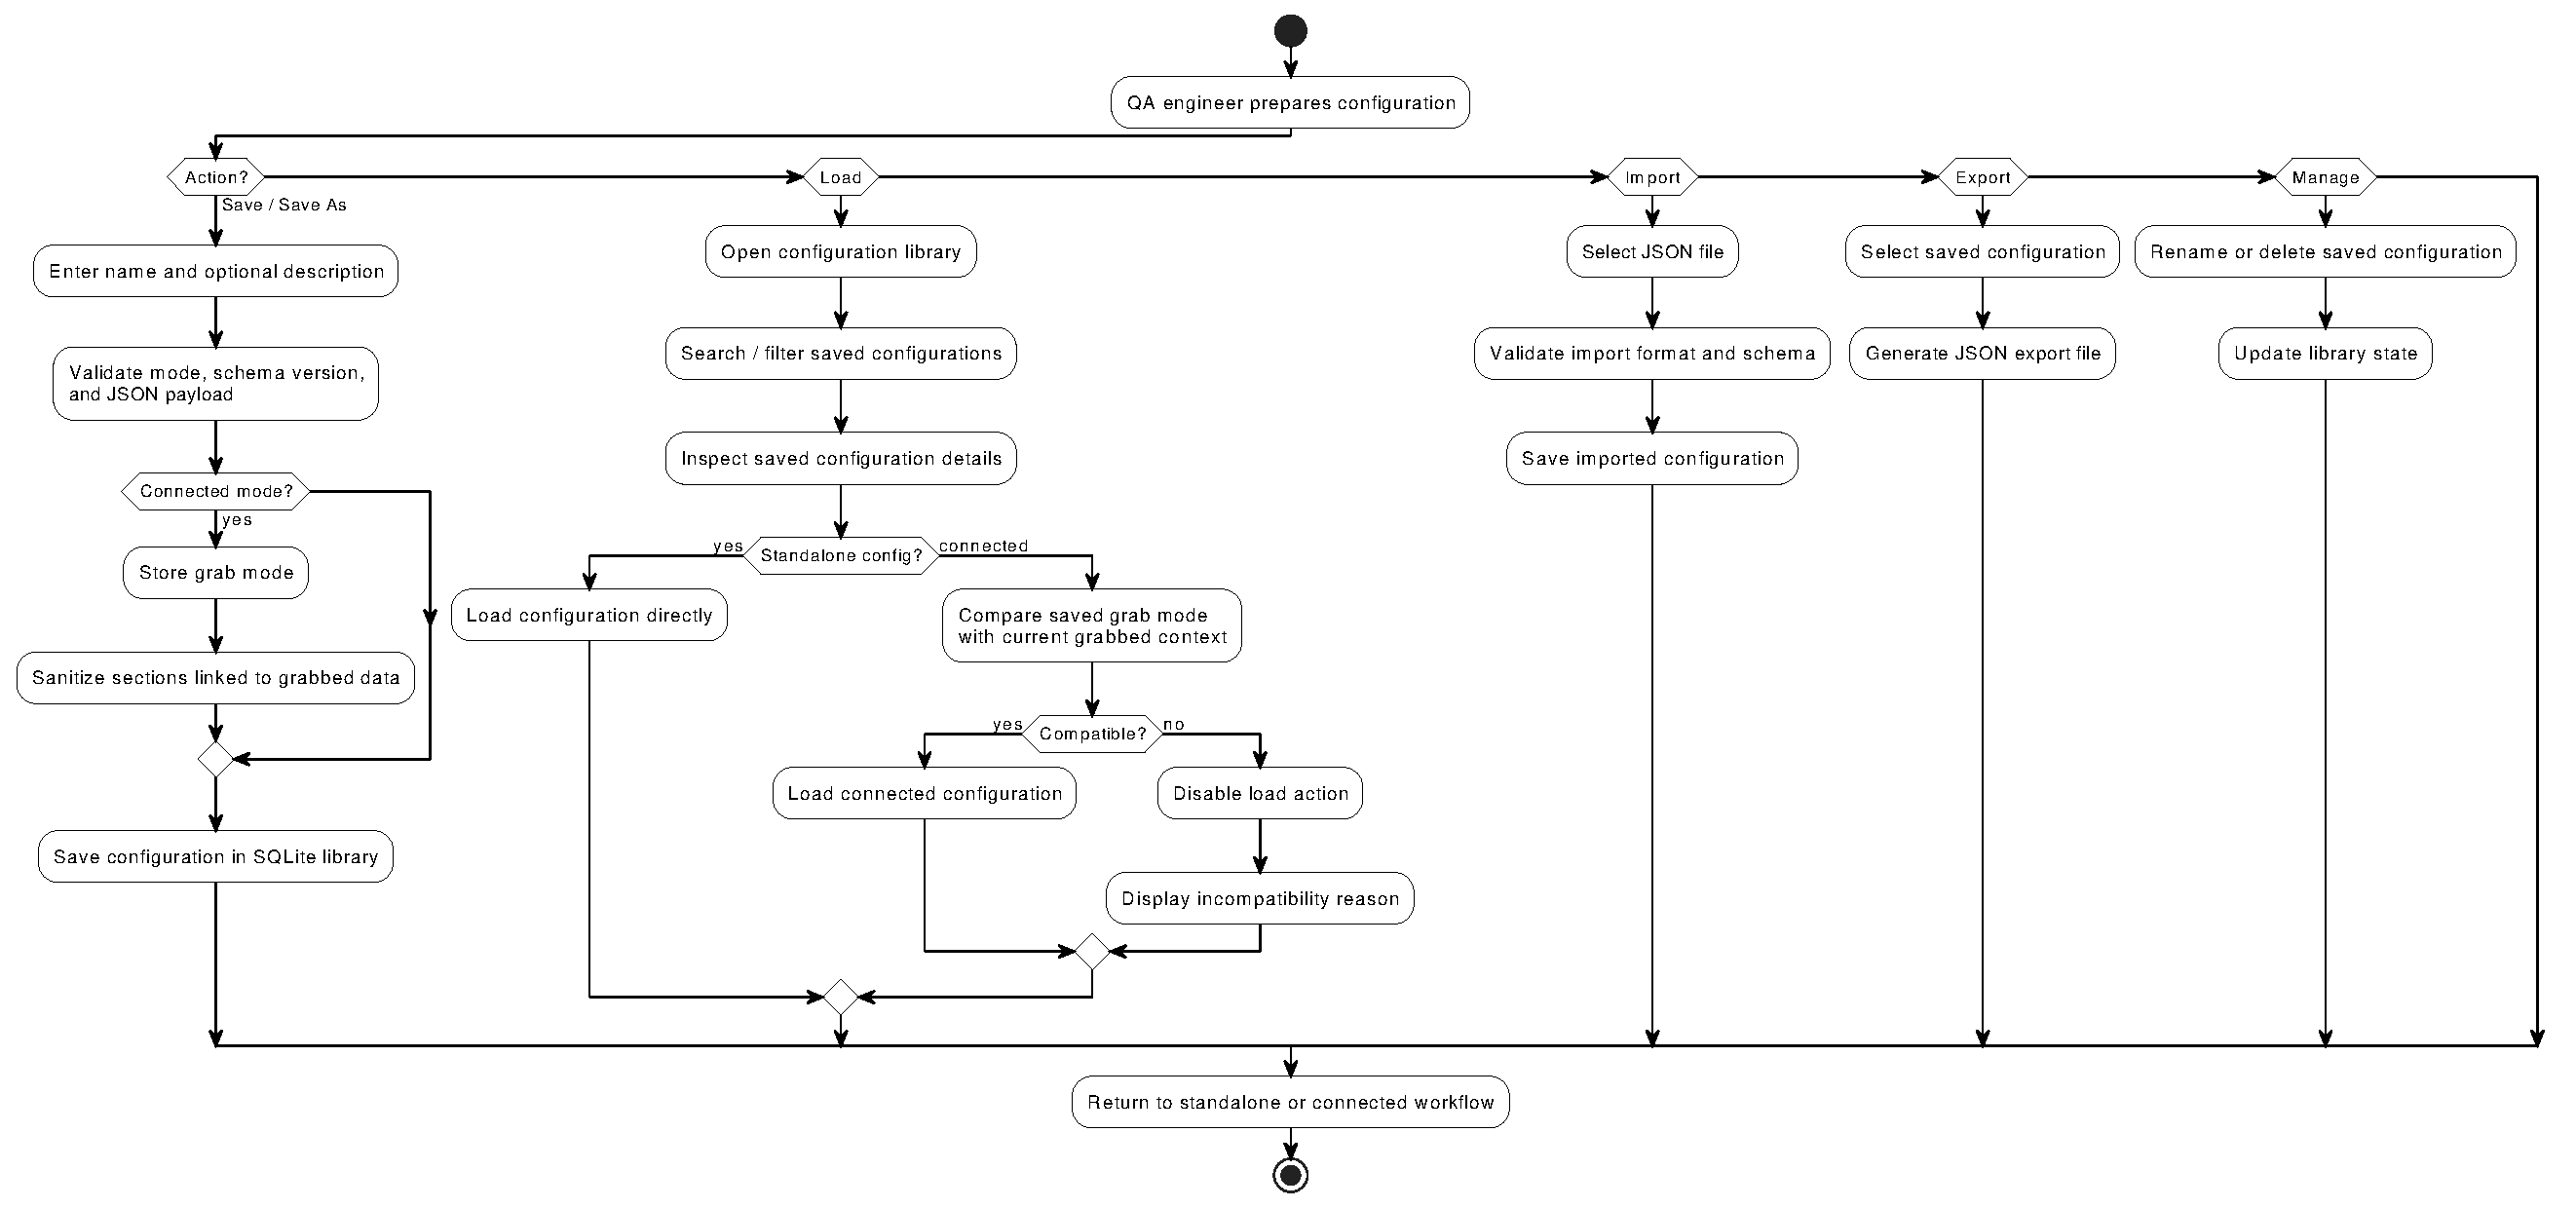
\includegraphics[width=0.86\textwidth]{img/activity-library.pdf}
\caption{Configuration library activity diagram}
\label{fig:activity-library}
\end{figure}

\subsection{Sequence Diagrams}

\paragraph{}Figure~\ref{fig:sequence-library} presents the main sequence of the configuration library.
It covers saving from a workflow, listing saved entries, loading a compatible scenario, updating or
overwriting metadata and payload, importing/exporting JSON, and deleting obsolete configurations.

\begin{figure}[!htbp]
\centering
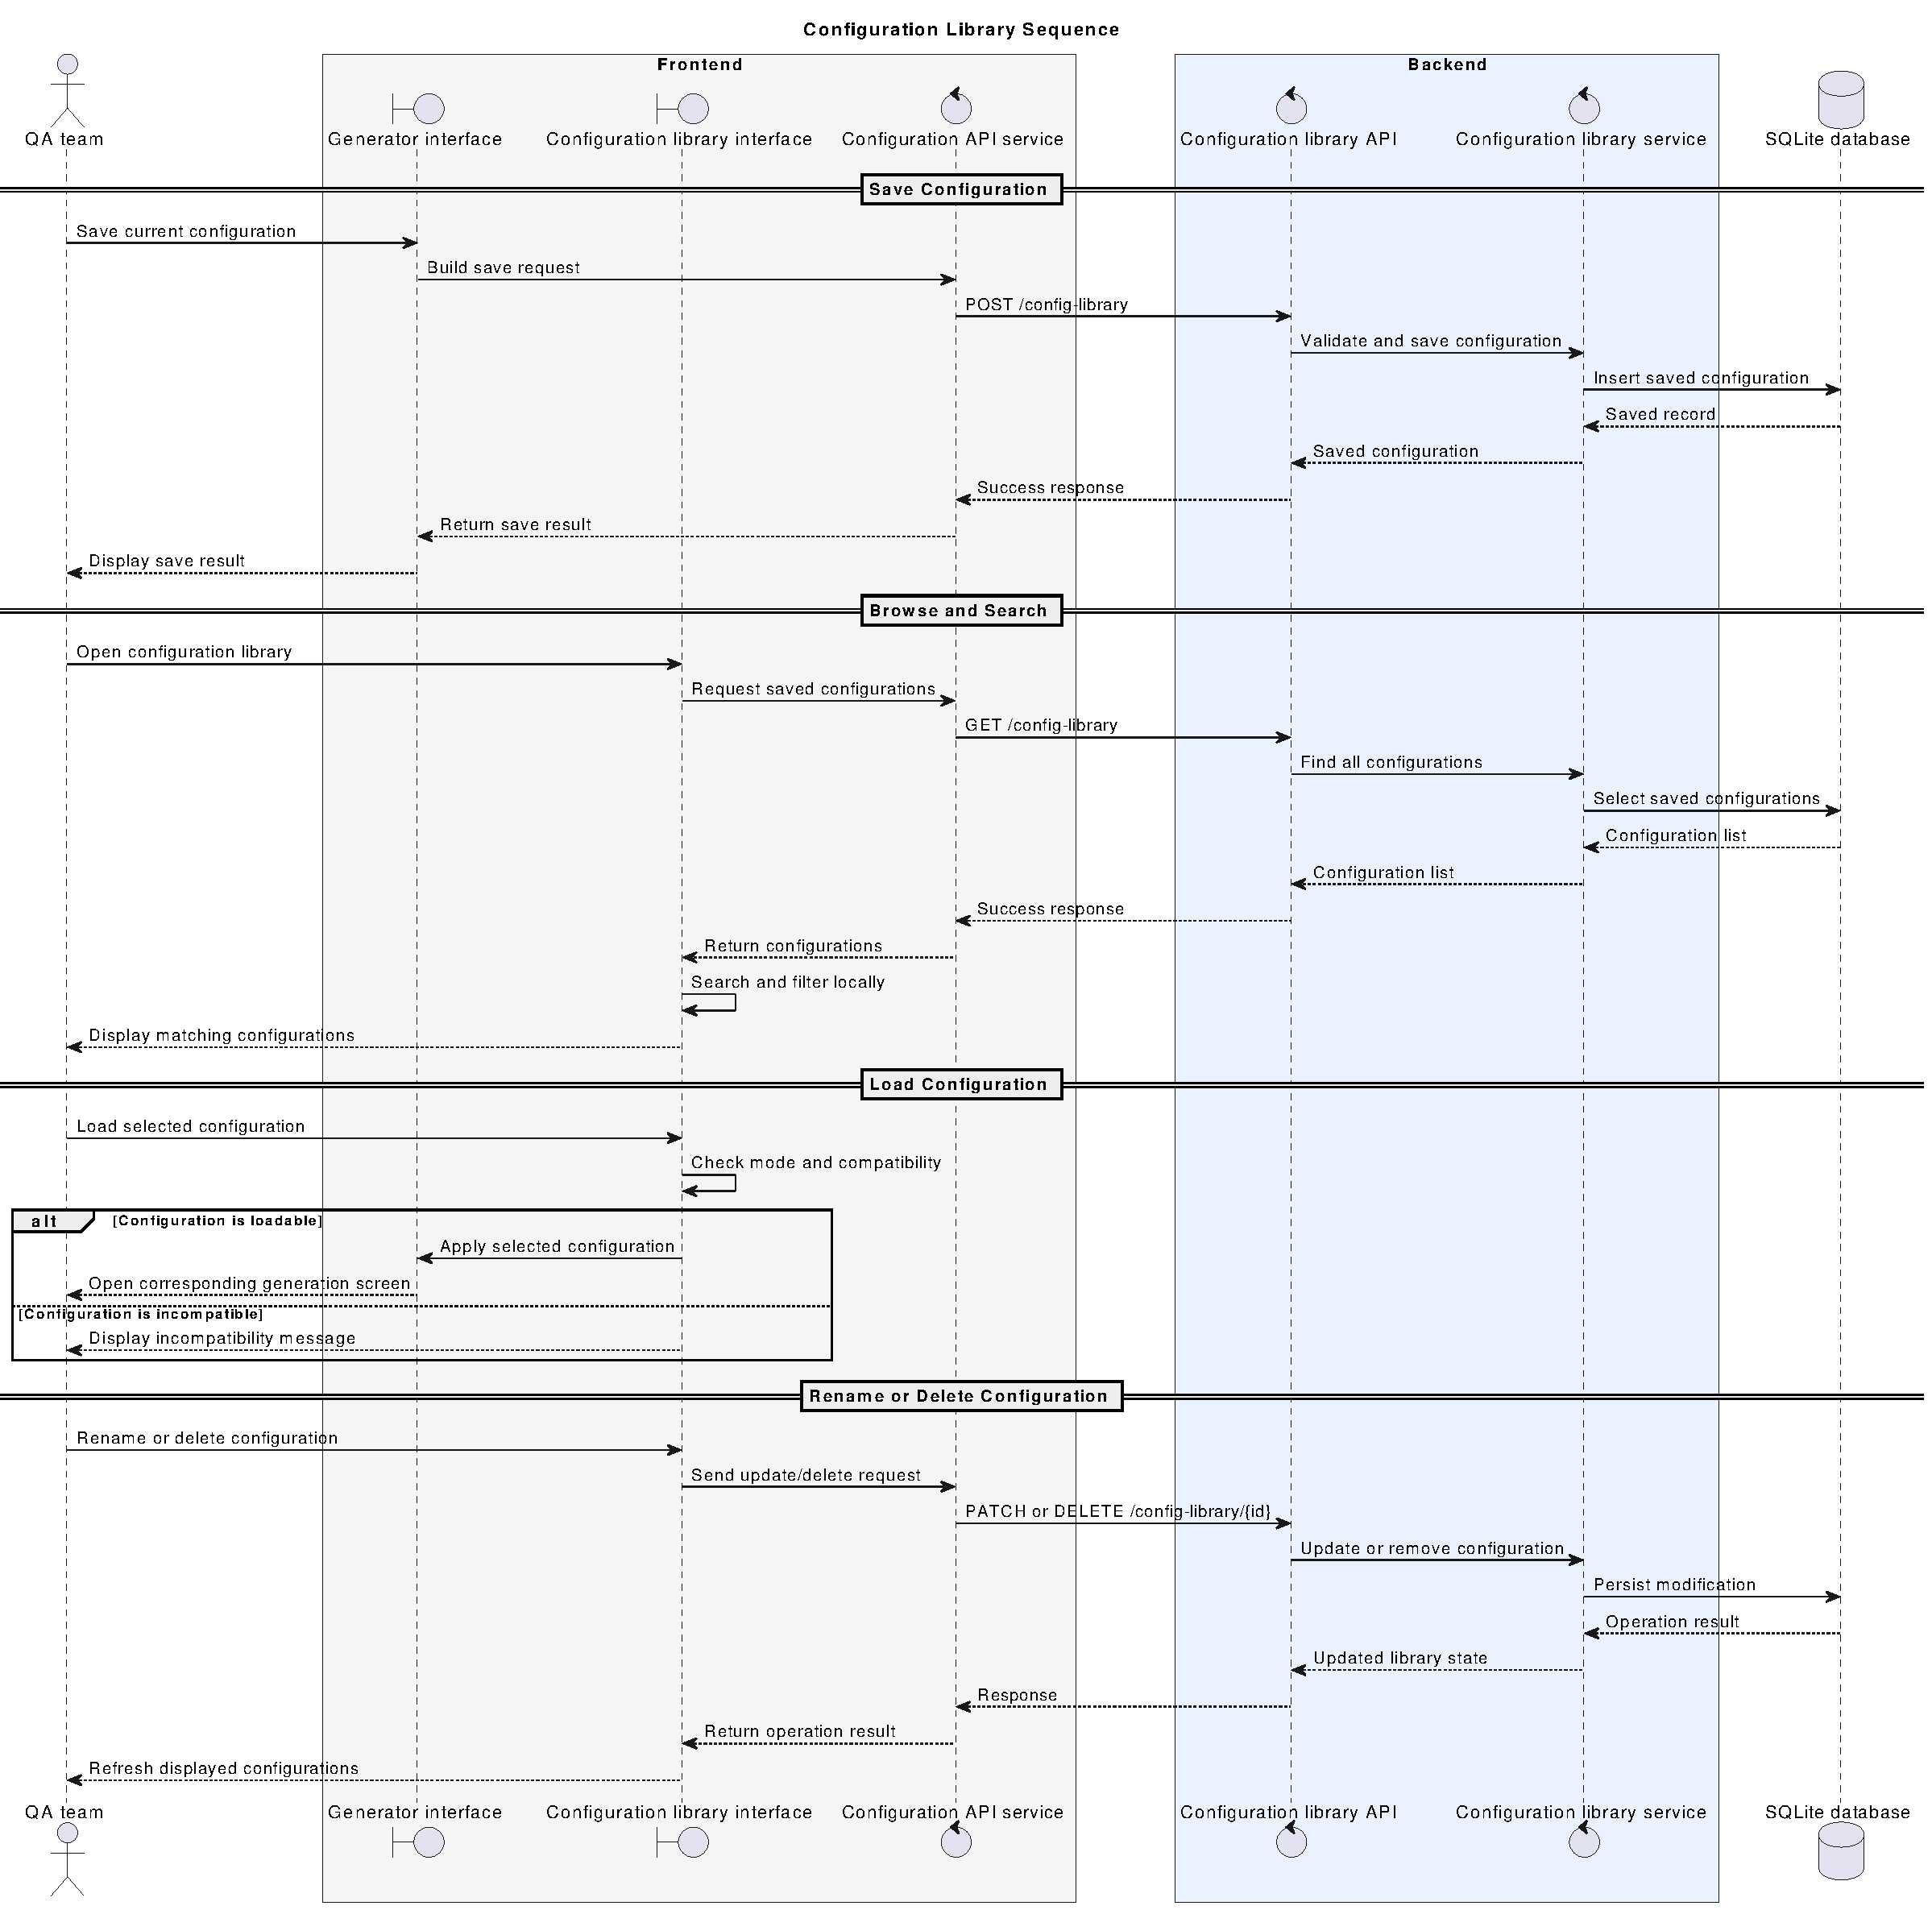
\includegraphics[width=0.95\textwidth]{img/sequence-configuration-library.pdf}
\caption{Configuration library sequence}
\label{fig:sequence-library}
\end{figure}

\section{Realization}

\paragraph{}Sprint 5 was implemented as a final workflow extension of the standalone and connected
modes. The application can now keep reusable scenarios in a local configuration library, restore
them into the correct workflow, and protect connected configurations from being loaded in the wrong
grabbed-data context.

\subsection{Configuration Library Realization Evidence}

\paragraph{}Table~\ref{tab:library-realization-proof} summarizes the proof of realization for Sprint 5.

\Needspace{13\baselineskip}
\renewcommand{\arraystretch}{1.3}
\begin{longtable}{|P{0.24\linewidth}|P{0.34\linewidth}|P{0.32\linewidth}|}
\caption{Configuration library realization evidence}
\label{tab:library-realization-proof} \\
\hline
\textbf{Evidence} & \textbf{Implemented result} & \textbf{Purpose} \\
\hline
\endfirsthead
\multicolumn{3}{r}{\tablename\ \thetable{} -- \textit{continued from previous page}} \\
\hline
\textbf{Evidence} & \textbf{Implemented result} & \textbf{Purpose} \\
\hline
\endhead
\hline
\multicolumn{3}{r}{\textit{continued on next page}} \\
\endfoot
\hline
\endlastfoot
Persistence & Saved configurations are stored through the \texttt{SavedConfig} entity and retrieved from the library API. & Proves that scenarios survive navigation and can be reused later. \\
\hline
Validation & Empty names, duplicate names, invalid modes, invalid grab modes, invalid schema versions, malformed JSON, and structurally invalid payloads are rejected. & Keeps the library clean and prevents unusable entries. \\
\hline
Schema versioning & Each saved entry and exported file includes a schema version. & Prepares the library for future configuration-format evolution. \\
\hline
Standalone reuse & A saved standalone payload is merged with default configuration values before being restored. & Allows old or partial saved configurations to remain usable. \\
\hline
Connected compatibility & Connected configs are filtered and disabled when they conflict with the current grabbed data. & Prevents duplicated accounts or securities and invalid dependent data. \\
\hline
Save lifecycle & The application tracks the loaded saved configuration and supports direct overwrite or Save As. & Lets QA engineers update existing scenarios without losing the option to create variants. \\
\hline
JSON exchange & Saved configurations can be exported as JSON and imported back into the library after validation. & Allows scenarios to be shared, archived, or moved between environments. \\
\hline
Expanded inspection & The eye action shows reference date, schema version, enabled sections, and estimated rows. & Helps the QA engineer choose the correct configuration before loading it. \\
\hline
Library management & The page supports search, mode filtering, details, import/export, overwrite, rename, deletion, loading state, empty state, and error state. & Provides a complete user-facing library workflow. \\
\hline
Navigation safeguard & Leaving an active connected session requires confirmation and resets the grabbed context after disconnecting. & Protects the QA engineer from mixing stale database context with a new workflow. \\
\hline
\end{longtable}
\renewcommand{\arraystretch}{1}

\subsection{User Workflow}

\paragraph{}The following figures show the implemented library screens and the final workflow proof.
The library is available from both standalone and connected workflows.

\paragraph{}Figure~\ref{fig:ch7-library-page} is reserved for the main library interface. It can be
completed with a screenshot showing saved cards, search, filters, import, details, export, overwrite,
and load actions.

\begin{figure}[!htbp]
\centering
\IfFileExists{img/ch7-library-page.png}{%
    \includegraphics[width=0.88\textwidth]{img/ch7-library-page.png}%
}{%
    \fbox{\parbox[c][0.22\textheight][c]{0.86\textwidth}{\centering Screenshot to be added: configuration library page with saved cards, search, filter, import, details, export, overwrite, and load actions}}%
}
\caption{Configuration library page}
\label{fig:ch7-library-page}
\end{figure}

\paragraph{}Figure~\ref{fig:ch7-library-proof} is reserved for proof of the final workflow. It can show
Save/Save As, direct overwrite confirmation, JSON import/export, expanded details, connected
compatibility feedback, or the disconnect safeguard.

\begin{figure}[!htbp]
\centering
\IfFileExists{img/ch7-library-proof.png}{%
    \includegraphics[width=0.88\textwidth]{img/ch7-library-proof.png}%
}{%
    \fbox{\parbox[c][0.22\textheight][c]{0.86\textwidth}{\centering Screenshot to be added: Save/Save As, overwrite confirmation, JSON import/export, expanded details, connected compatibility, or disconnect safeguard}}%
}
\caption{Configuration library and final workflow evidence}
\label{fig:ch7-library-proof}
\end{figure}

\section*{Conclusion}
\addcontentsline{toc}{section}{Conclusion}

\paragraph{}Sprint 5 finalized the Longview Test Data Generator by adding a complete saved-configuration
lifecycle and workflow safeguards. The application now supports standalone generation, connected
generation, optional enrichment, SQL export, saved scenario reuse, Save/Save As, direct overwrite,
JSON import/export, connected compatibility checks, and protected navigation for active connected
sessions.
